\section{溶液濃度の影響}

先ほどの節では,密度による落下球高速化への影響を議論したが,本節では溶液濃度による高速化への影響に関して考える.

PAA溶液濃度と終端速度の関係をFig.\ref{fig:concentrationUT}に示す.溶液濃度が濃くなると,終端速度が遅くなることが分かった.

PAA溶液濃度と高速化度合の関係をFig.\ref{fig:concentrationUdiff}に示す.縦軸は高速化度合$U_\text{on}/U_\text{off}$,横軸はPAA溶液濃度である.

式(\ref{eq:UdiffRho})を用いて

\begin{figure}[ht]
    \centering
    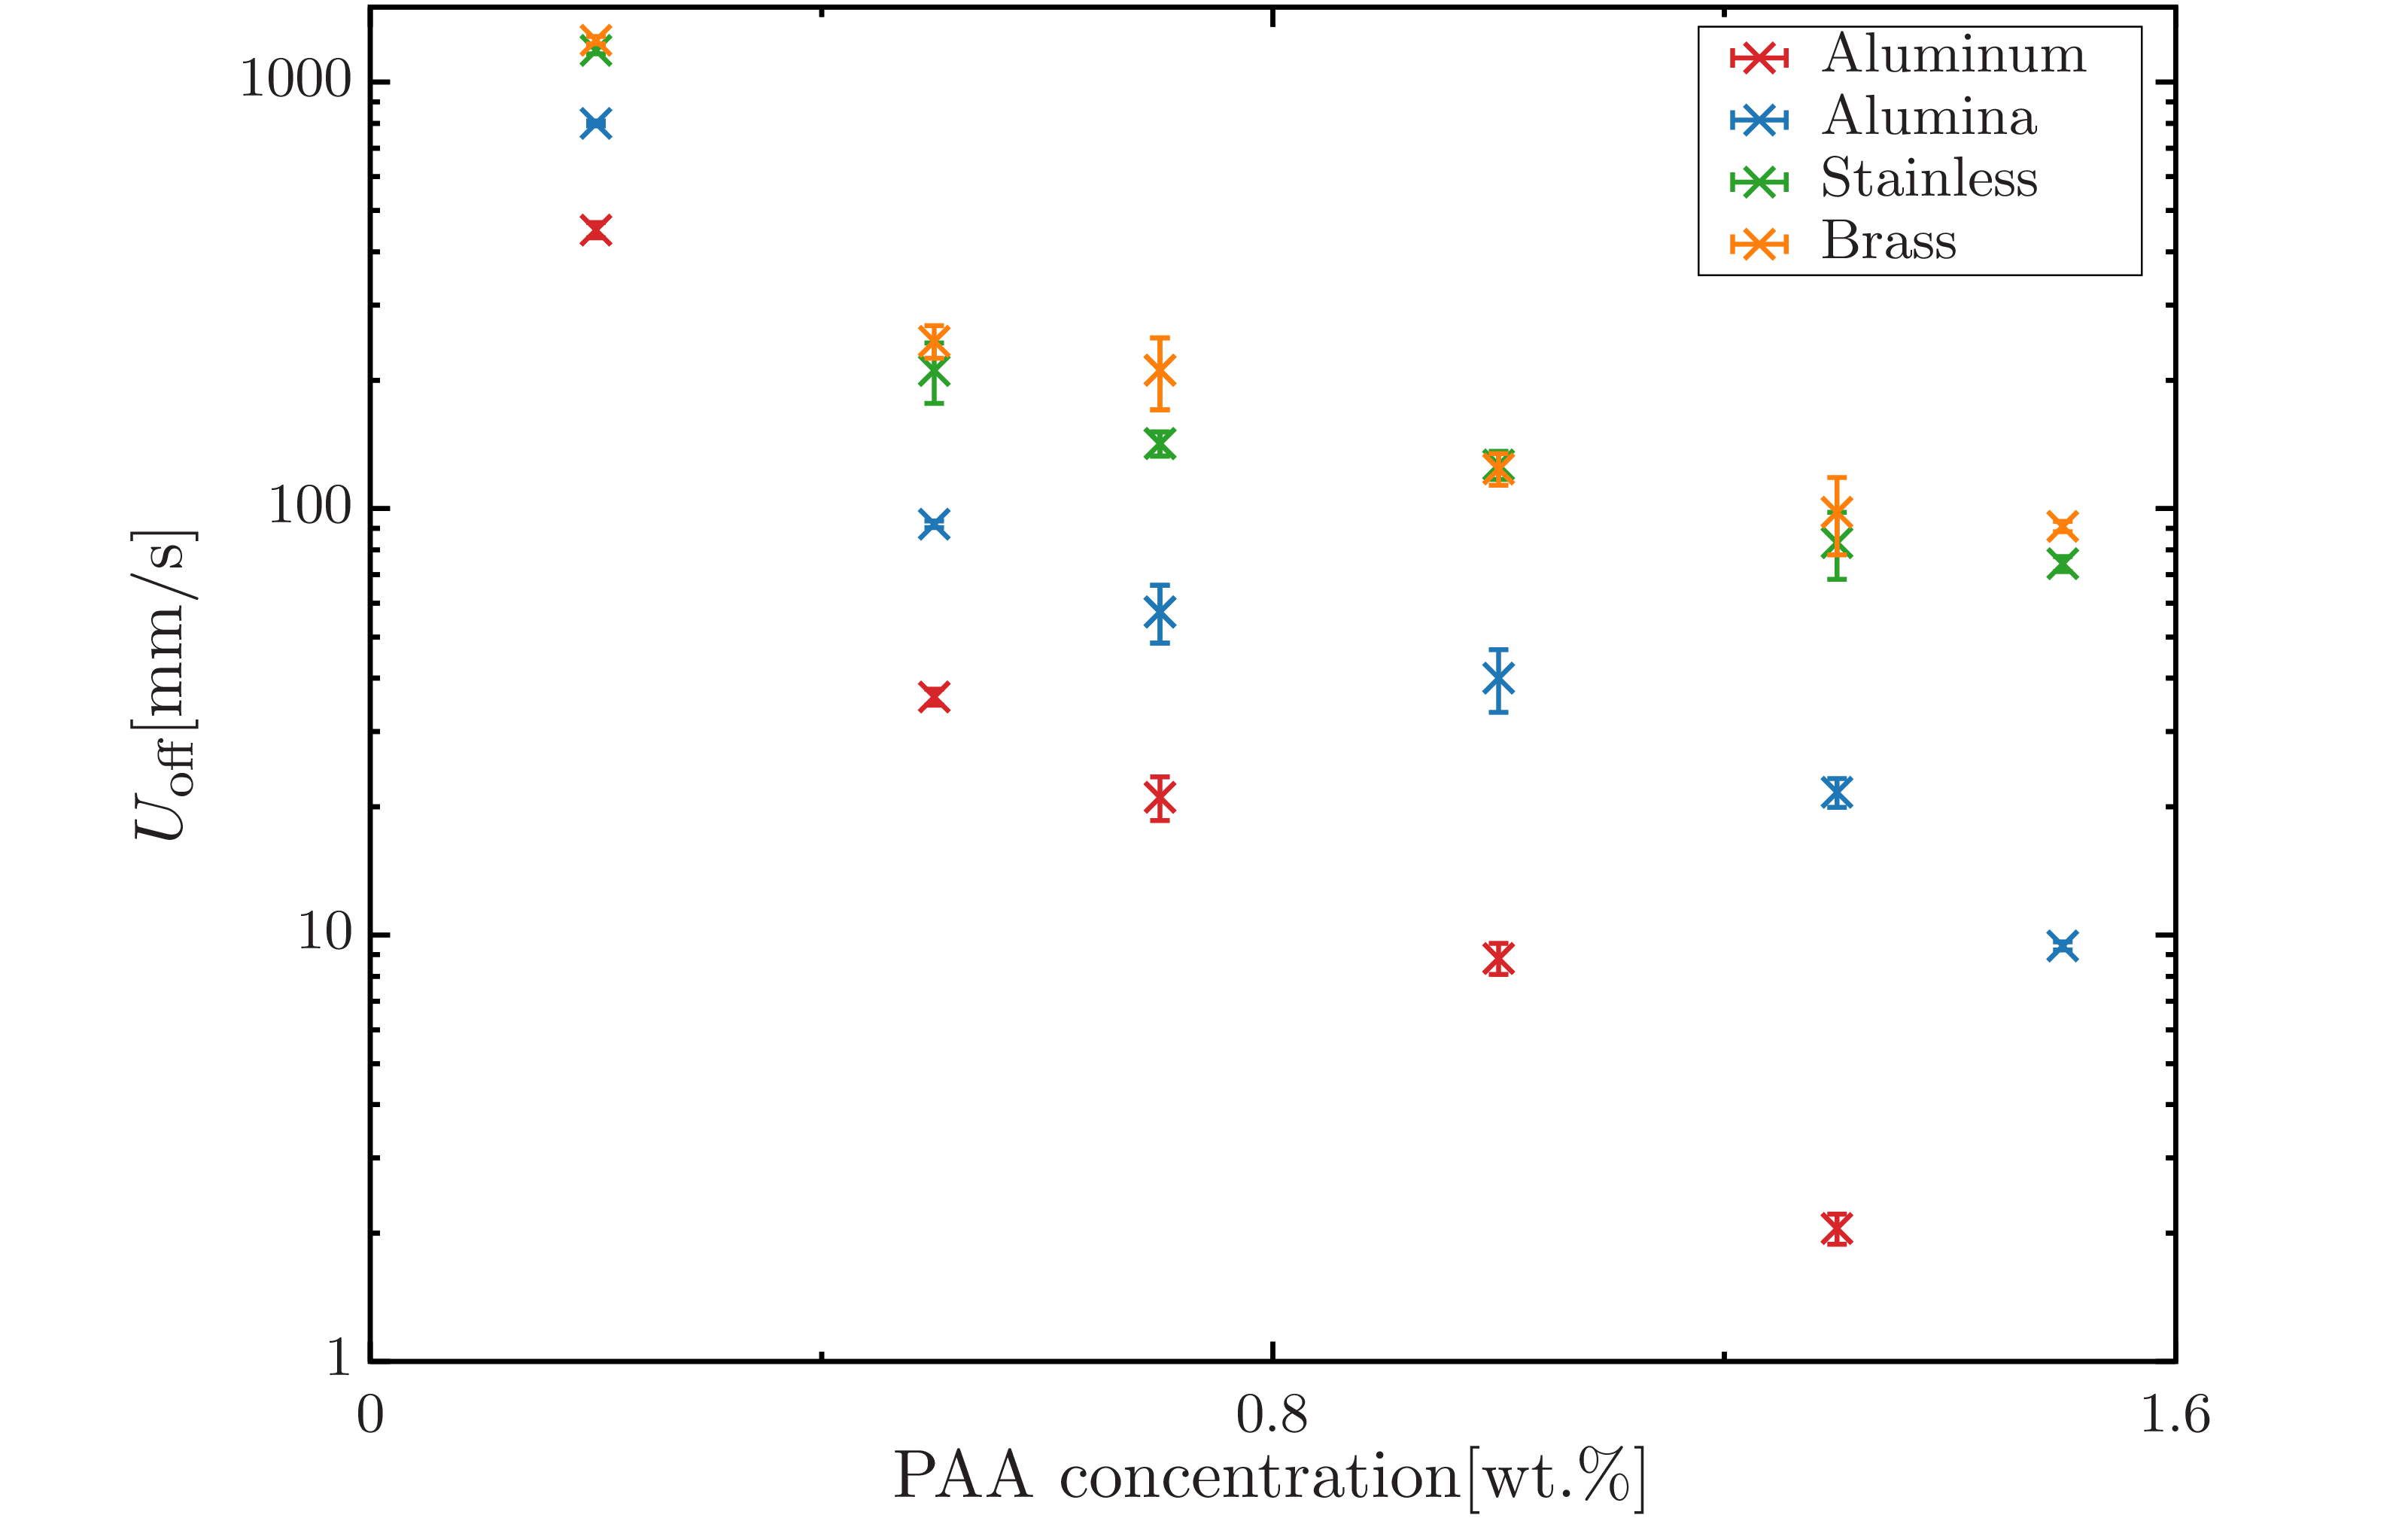
\includegraphics[width=1.0\textwidth]{./5-Results/concentration/concentrationUT.png}
    \caption{Termination velocity in PAA solution concentration.}
    \label{fig:concentrationUT}
\end{figure}

\begin{figure}[ht]
    \centering
    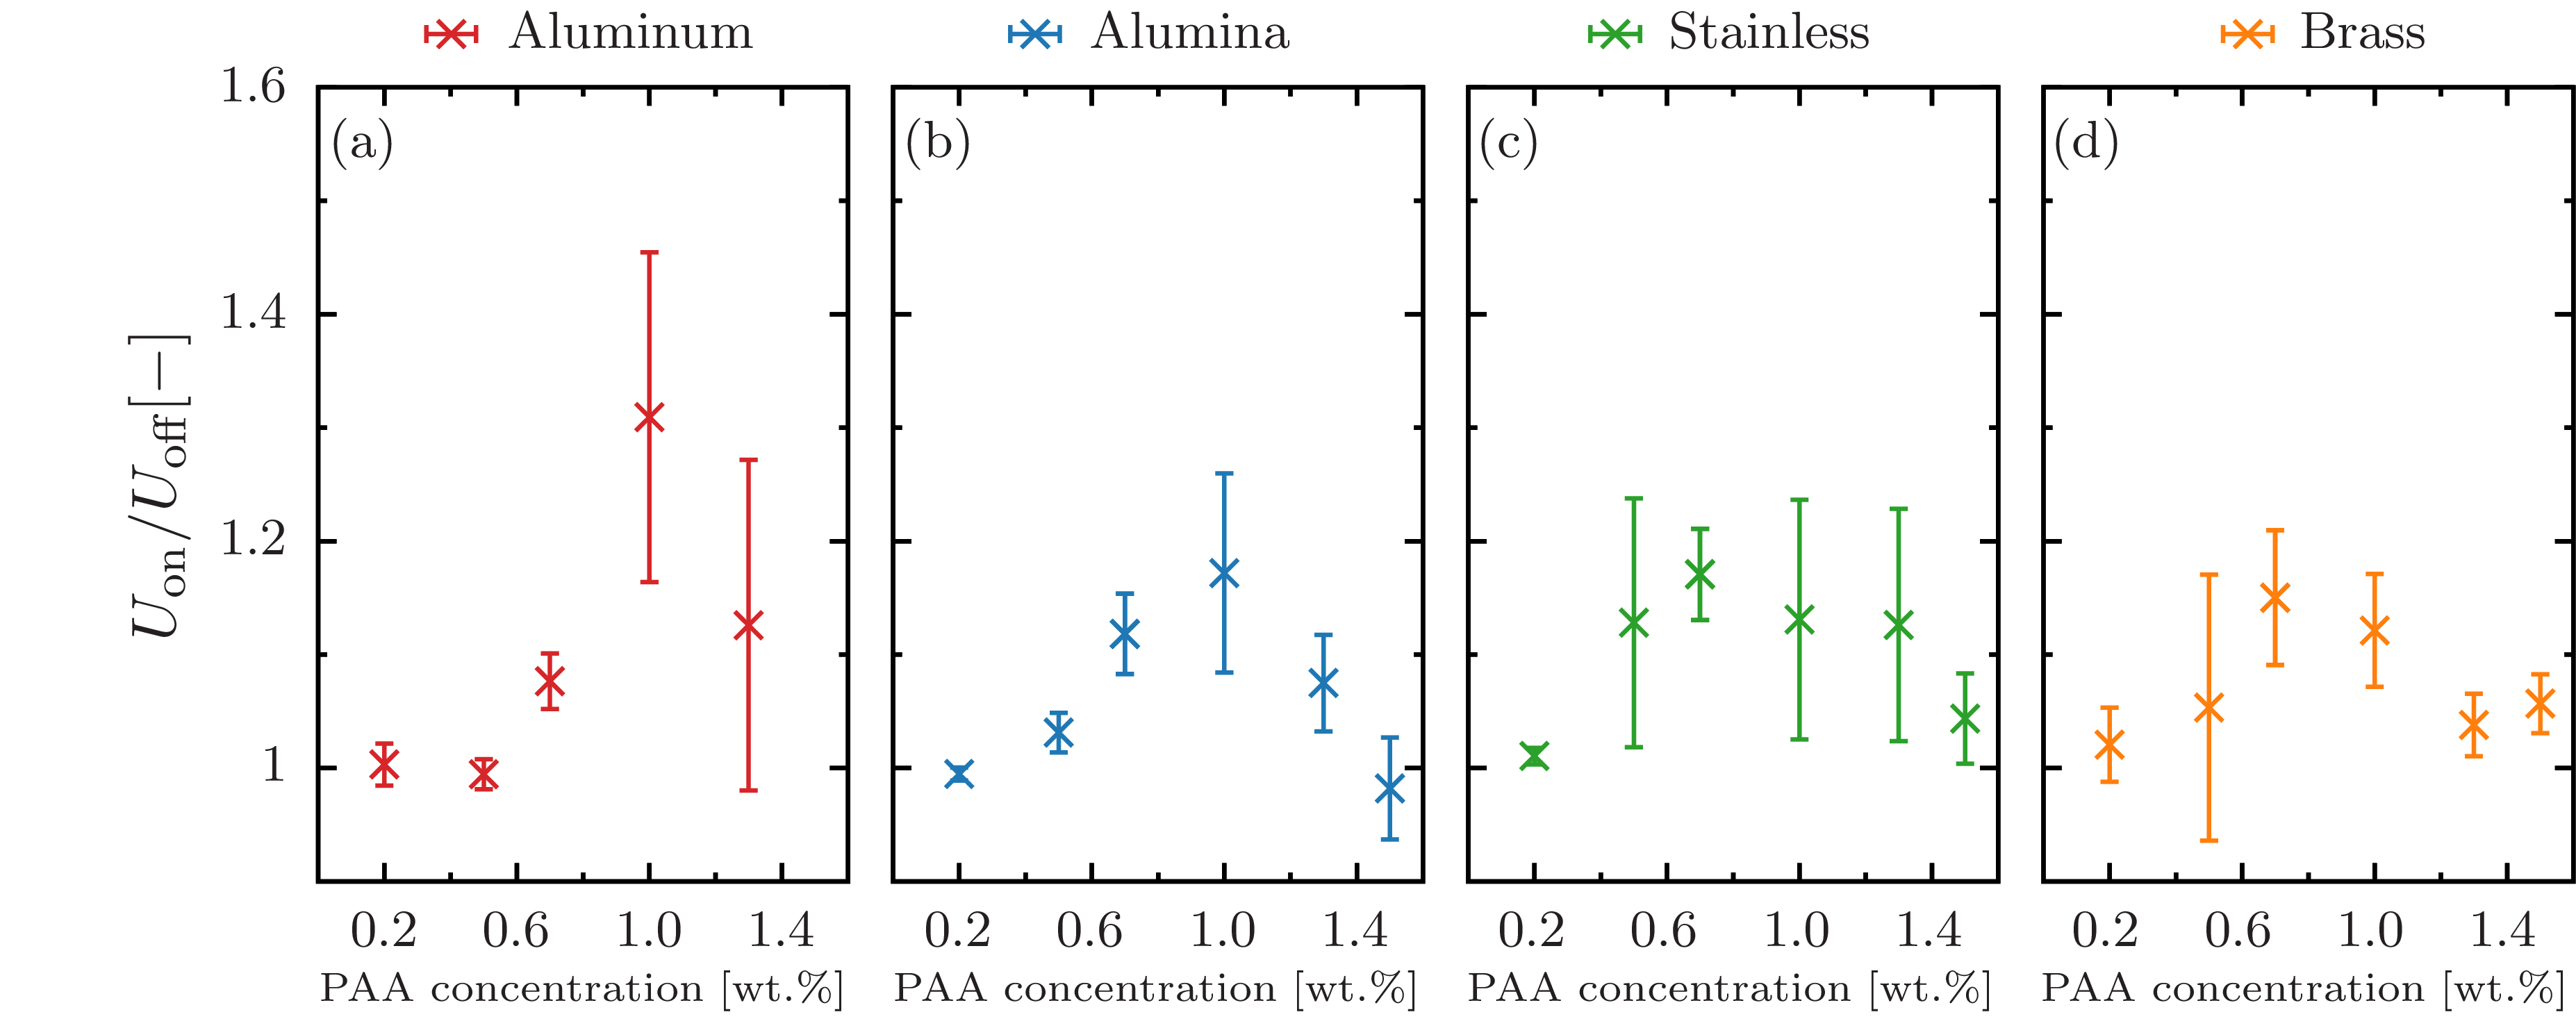
\includegraphics[width=1.0\textwidth]{./5-Results/concentration/concentrationUdiff.png}
    \caption{Velocity ratio in PAA solution concentration (a)Aluminum, (b)Alumina, (c)Stainless, (d)Brass.}
    \label{fig:concentrationUdiff}
\end{figure}

\begin{figure}[ht]
    \centering
    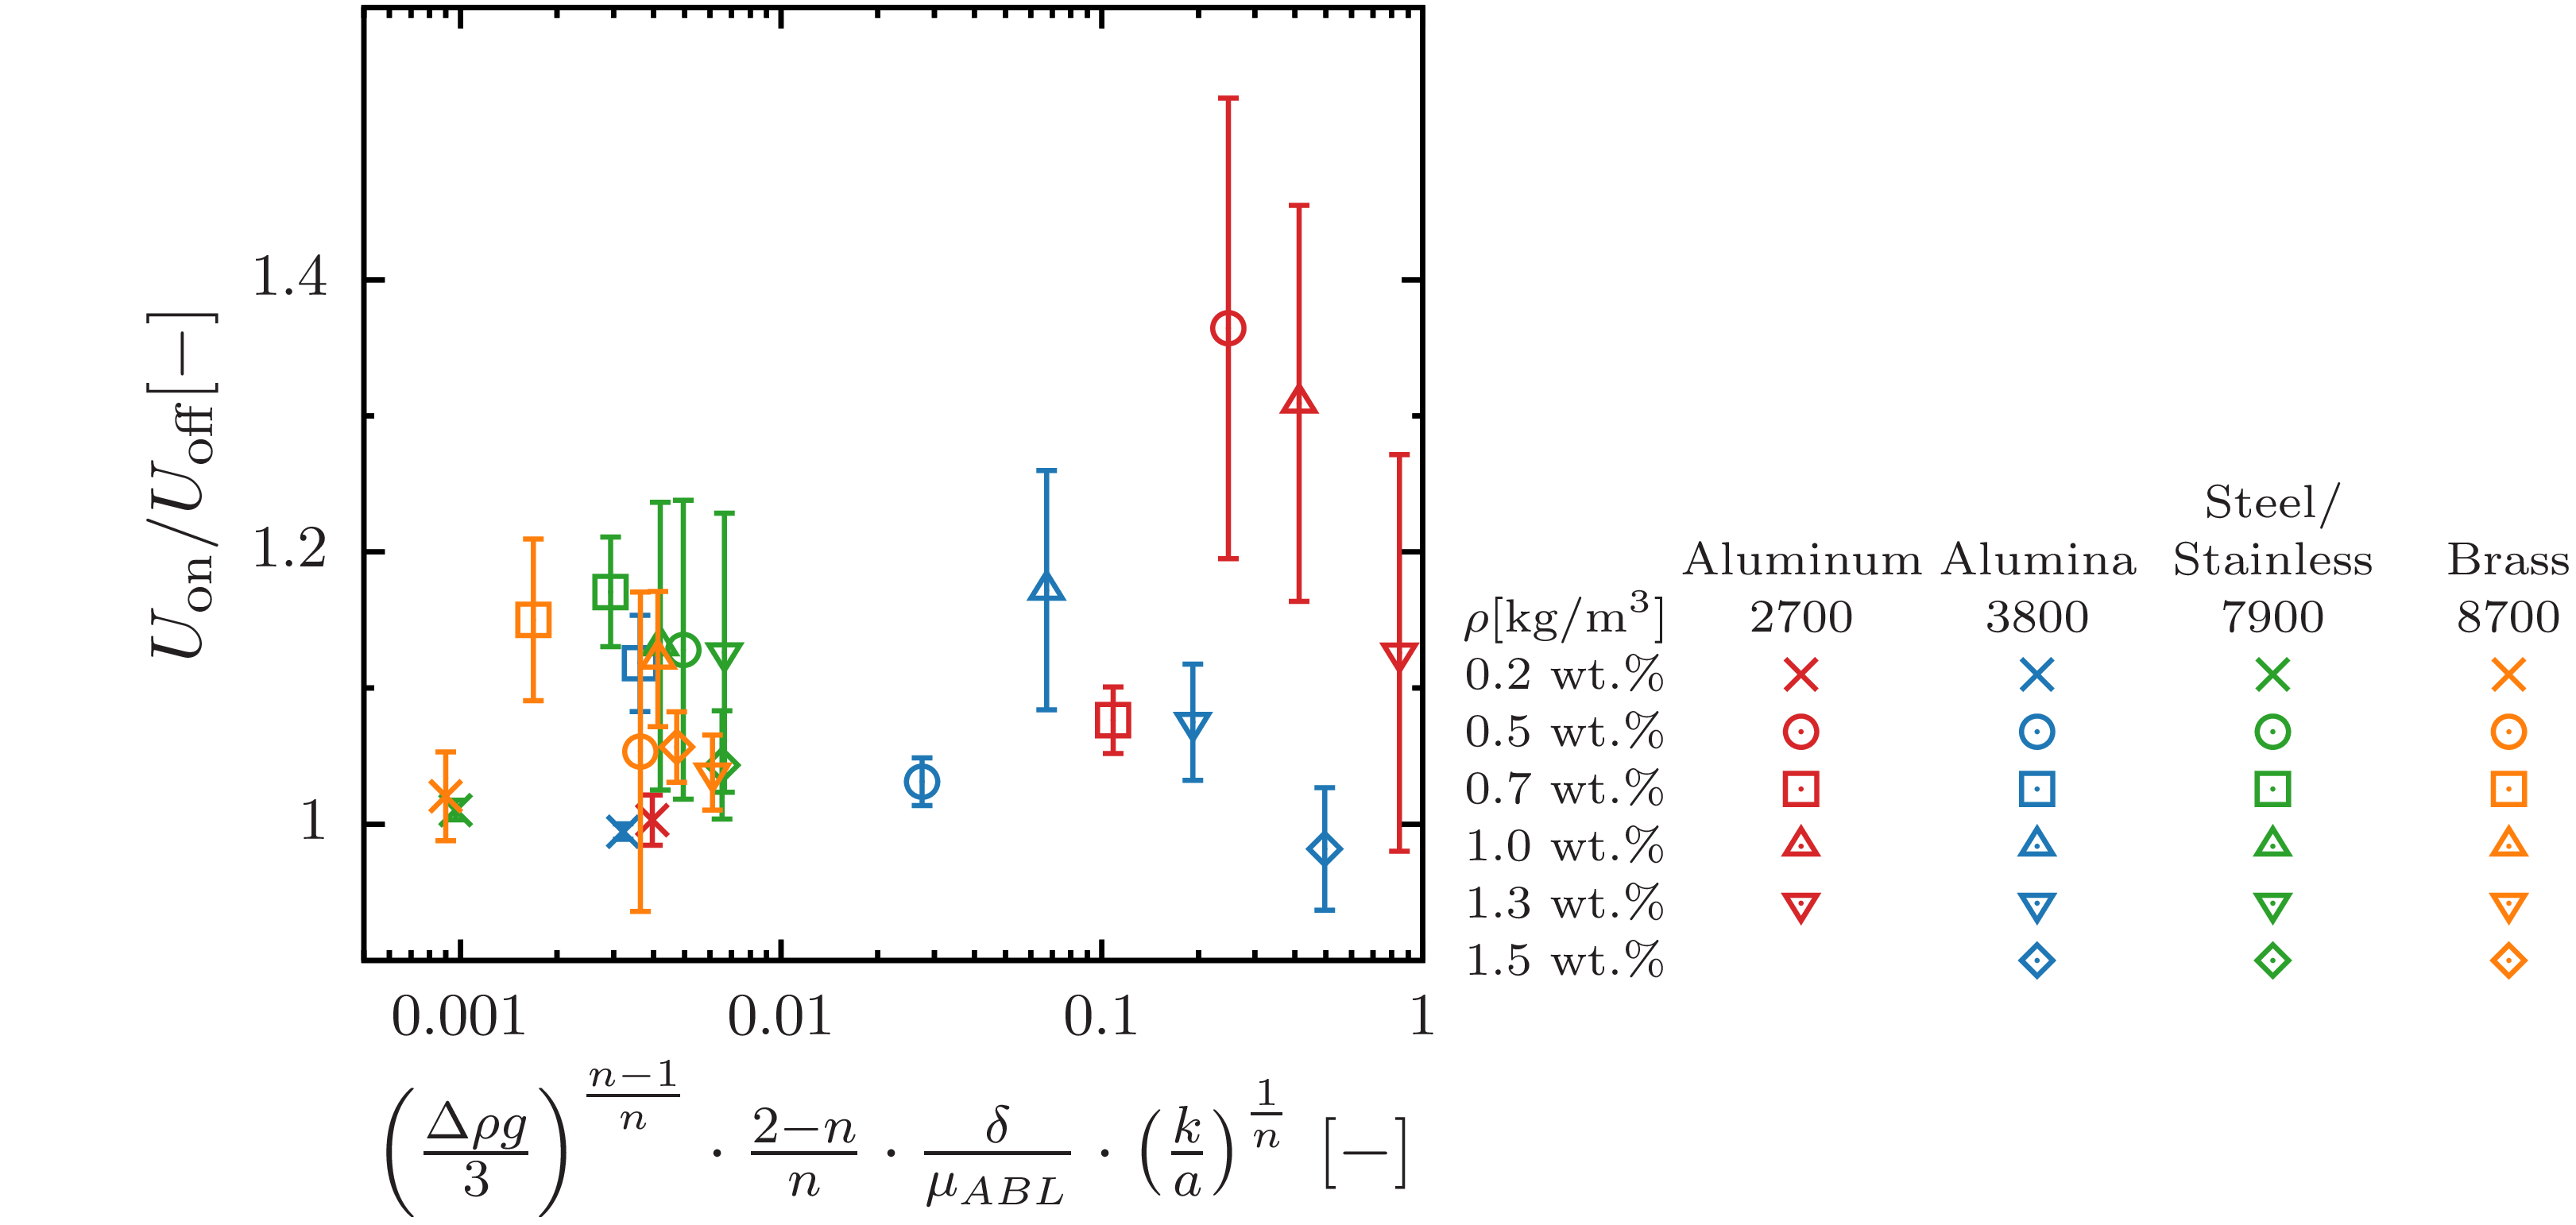
\includegraphics[width=1.0\textwidth]{./5-Results/concentration/concentrationUdiffAll.png}
    \caption{}
    \label{fig:concentrationUdiffAll}
\end{figure}